\documentclass[letterpaper,11pt]{article}
\pdfoutput=1

\usepackage[margin=2cm]{geometry}
\usepackage{graphicx}

\begin{document}

\begin{figure}
  \centering
  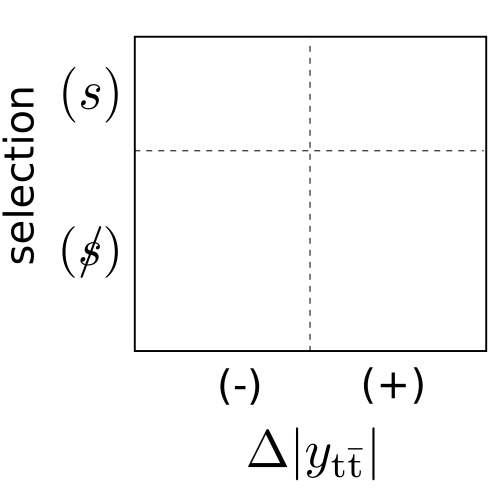
\includegraphics[width=0.3\linewidth]{axes}
  \caption{\label{axes} Four bins, selected (A) and unselected (B) on
    the selection axis, and $(-)$ and $(+)$ on the axis of the the
    observable for which the asymmetry is of interest.}
\end{figure}

\section{Demonstration of technique failures}

Consider a two dimensional distribution of four bins, where one axis
is a selection observable with bins (selected, A) and (unselected, B),
and the other is an observable for which the asymmetry is of interest,
for example $\Delta|y_{\mathrm{t\bar{t}}}|$, with bins $(+)$ and
$(-)$.  Figure \ref{axes} shows the axes. In a model $N$, the
selection contains $N_A$ events and has asymmetry $\alpha_A$, while
the unselected events number $N_B$ and may have a different asymmetry
$\alpha_B$.  The counts in each bin of the model are given by
\[N_x^{\pm} = N_x(1\pm\alpha_x)/2,\]
where $N_x=N_x^-+N_x^+$, and the total asymmetry is given by
\[\alpha = \frac{N_A\alpha_A + N_B\alpha_B}{N_A+N_B}.\]
Note that $\alpha_A\ne\alpha_B$ implies that the selection
efficiencies for the bins $(+)$ and $(-)$ are unequal.

Suppose we want to measure the asymmetry of an alternative model $D$
which has an antisymmetric component proportional to that of model
$N$, with factor $F$,
\[D_x^{\pm} = N_x(1\pm F\alpha_x)/2,\]
and where we suppose that $D_x=N_x$.  The total asymmetry in model $D$
would be $F\alpha$.


\subsection{Template Strategy}
Following the template strategy we have so far employed, the weights
which symmetrize and antisymmetrize the original distribution after
integrating over the selection axis would be
\[W^\pm_{\mathrm{symm}} = (1\pm\alpha)^{-1},\]
\[W^\pm_{\mathrm{anti}} = \pm\alpha(1\pm\alpha)^{-1}.\]
The templates for the selection would be
\[T^{\pm}_{\mathrm{symm}} = \frac{N_A}{2}\frac{1\pm\alpha_A}{1\pm\alpha},\]
\[T^{\pm}_{\mathrm{anti}} = \pm\alpha\frac{N_A}{2}\frac{1\pm\alpha_A}{1\pm\alpha},\]
and the parametrized template model would be
\[T^{\pm}(f) = T^{\pm}_{\mathrm{symm}} + f\cdot T^\pm_{\mathrm{anti}} = \frac{N_A}{2}\frac{1\pm\alpha_A}{1\pm\alpha}(1\pm f\cdot\alpha).\]
Our expectation has been that $T^\pm(f) = D^\pm_A$ when $f=F$, but
that is clearly only the case if $F=f=1$ or $\alpha=\alpha_A$.  The
former condition is useless for a measurement, while the latter
condition is generally unmet, and is particularly untrue in the cases
of our subselections at extremes of $\mathrm{t\bar{t}}$ system
rapidity and mass.

\subsection{Unfolding Strategy}
The ratios $R_N^{\pm}=N^{\pm}_A/N^{\pm}_B$ given by the model are used
to calculate the corresponding unselected bins
\[U^{\pm}_B = D^{\pm}_A/R^\pm_N = D^\pm_B\left(\frac{1\pm\alpha_A}{1\pm\alpha_B}\right)\]
The expectation that $U^\pm_B=D^\pm_B$ is not met, leading to a
mistake in calculating a corresponding total asymmetry
\begin{eqnarray*}
  \alpha' &=& \frac{D^+_A+U^+_B - D^-_A -
    U^-_B}{D^+_A+U^+_A+D^-_A+U^-_B}\\
  %&=& F \cdot \left(\frac{N_A\alpha_A + N_B\left[\alpha_A\left(\frac{1-\alpha_A\alpha_B}{1-\alpha_A^2}\right) + \frac{1}{F}\left(\frac{\alpha_B-\alpha_A}{1-\alpha_A^2}\right)\right]}{N_A+N_B\left[\left(\frac{1-\alpha_A\alpha_B}{1-\alpha_A^2}\right)+F\alpha_A\left(\frac{\alpha_B-\alpha_A}{1-\alpha_A^2}\right)\right]}\right)\\
  &=& F \alpha_A\cdot \left(\frac{N_A/N_B + \left[(1-\alpha_A\alpha_B) + \left(\frac{\alpha_B}{\alpha_A}-1\right)/F\right]/(1-\alpha_A^2)}{N_A/N_B+\left[\left(1-\alpha_A\alpha_B\right)+F\alpha_A\left(\alpha_B-\alpha_A\right)\right]/(1-\alpha_A^2)}\right)
\end{eqnarray*}
As an example of the significant measurement errors which can be
introduced by this flawed calculation, consider the plausible case
$\alpha_A=0\ne\alpha_B$.  We would find $\alpha' = \alpha \ne F\alpha$.

In the {\sc POWHEG} $\mathrm{t\bar{t}}$ simulation of CMS events
(model $N$, suppose), we have $\alpha=A_c^y\approx0.0056$, a selection
efficiency in lepton+jets channels of $N_A/(N_A+N_B)\approx 0.05$,
$\alpha_A\approx0.0032$, which implies $\alpha_B\approx0.0057$ and
$N_A/N_B\approx0.052$.  The true asymmetry in model $D$, given by
$F\alpha$, and the asymmetry $\alpha'$ calculated by unfolding model
$D$ using ratios $R_N^\pm$, are plotted in Figure \ref{plot} as a
function of the scale factor $F$.  We see that $\alpha'$ and $F\alpha$
have very different slopes as a function of $F$, and coincide only for
$F=1$, when models $N$ and $D$ coincide.
\begin{figure}
  \centering
  \includegraphics[width=0.5\textwidth]{plot}
  \caption{\label{plot} Modeled $A_c^y$ and its calculation from a CMS
    lepton+jets subselection via unfolding, as a function of the
    amplitude $F$ of the {\sc POWHEG} antisymmetric component.  Only
    when $F=1$ does the unfolding procedure yield the correct result.}
\end{figure}

\end{document}
